% interactcsesample.tex
% v1.05 - August 2017

\documentclass[]{interact}

\usepackage{epstopdf}% To incorporate .eps illustrations using PDFLaTeX, etc.
\usepackage[caption=false]{subfig}% Support for small, `sub' figures and tables
%\usepackage[nolists,tablesfirst]{endfloat}% To `separate' figures and tables from text if required

%\usepackage[doublespacing]{setspace}% To produce a `double spaced' document if required
%\setlength\parindent{24pt}% To increase paragraph indentation when line spacing is doubled
%\setlength\bibindent{2em}% To increase hanging indent in bibliography when line spacing is doubled

\usepackage{natbib}% Citation support using natbib.sty
\bibpunct[, ]{(}{)}{;}{a}{}{,}% Citation support using natbib.sty
\renewcommand\bibfont{\fontsize{10}{12}\selectfont}% Bibliography support using natbib.sty

\theoremstyle{plain}% Theorem-like structures provided by amsthm.sty
\newtheorem{theorem}{Theorem}[section]
\newtheorem{lemma}[theorem]{Lemma}
\newtheorem{corollary}[theorem]{Corollary}
\newtheorem{proposition}[theorem]{Proposition}

\theoremstyle{definition}
\newtheorem{definition}[theorem]{Definition}
\newtheorem{example}[theorem]{Example}

\theoremstyle{remark}
\newtheorem{remark}{Remark}
\newtheorem{notation}{Notation}

\begin{document}

\articletype{ARTICLE}% Specify the article type or omit as appropriate

\title{The responses of \textit{Spinifex littoreus} to sand burial on the coastal area of Pingtan Island, Fujian Province, South China}

\author{
\name{
  Shuang Song\textsuperscript{a}, 
  Jianhui Du \textsuperscript{a,b} \thanks{CONTACT Jianhui Du. Email: dujh1982@hotmail.com}, 
  Qirui Wu \textsuperscript{a},
  Mingyang Ni \textsuperscript{a} and Yingling Zhang \textsuperscript{a}}\affil{\textsuperscript{a}School of Geography and Planning, Sun Yat-Sen University, Guangzhou, 510275, China; \textsuperscript{b} Guangdong Key Laboratory for Urbanization and Geo-simulation, Guangzhou, 510275, China}
}

\maketitle

\begin{abstract}
\label{abstract}
% 砂生植物对沙埋藏的适应能力对海岸沙丘系统的生态恢复至关重要。
The adaptive capacity of psammophytes to sand burial is crucial for the ecological restoration of coastal dune systems. 
% 研究了福建平潭岛海岸滨鹬对不同埋沙深度和埋沙深度的响应。
The responses of Spinifex littoreus to different sand burial depths and levels were examined on the coast of Pingtan island, Fujian Province, South China. 
% 结果表明,与对照组相比,砂埋对其匍匐茎的垂直生长无显著影响。
The results indicated that, compared to the control group, sand burial on the S. littoreus stolons had no significant impact on its vertical growth of conjoint ramets. 
% 随着砂埋的继续,匍匐茎顶端生长更快,完全砂埋比半砂埋影响更明显。
The stolon apex grew even faster as the sand burial continued, with more obvious influence under complete sand burial than half sand burial. 
% 不同埋沙处理均能刺激和产生荔枝匍匐茎上的不定根,其长度随埋沙水平的变化而变化。
Adventitious roots on S. littoreus stolons were stimulated and produced in all sand burial treatments, the length of which varied according to the sand burial levels. 
% 在不定根和叶片上,三个匍匐茎上的干生物量分配均发生了变化,而在茎上则没有变化。
Dry biomass allocation were altered by sand burial in both adventitious roots and leaves, but not in stems. 
More adventitious roots on base of stolon and leaves on apex of stolon were observed. 
% 通过匍匐茎的快速生长,匍匐茎基部产生大量不定根,匍匐茎顶端的叶片萌发率较高,可以适应完全的砂埋。
S. littoreus can adapt to complete sand burial by rapid growth of stolons, abundant production of adventitious roots on the stolon base, and more germination of leaves on the stolon apex.
\end{abstract}

\begin{keywords}
Psammophytes; sand burial; \textit{Spinifex littoreus}; responses, plant osmotic stress
\end{keywords}


\section{Introduction}

\label{Introduction-1}
% 主要介绍沙生植物对海岸生态系统对重要意义
Sand dunes occupy a finite area in coastal regions, but they are characterized by providing multiple ecological services, and play an important role in the sustainable development in those regions with rising sea levels, surface subsidence and coastal hazards (Martínez et al. 2004, De Battisti \& Griffin 2020). Recently, due to the influence of both climate change and anthropogenic activities, many coastal sand dunes have been modified or destroyed, and this can, or has potentially led to the retreat of coastlines, disappearance of habitats, loss of biodiversity, and severe degradation of ecosystem functions in coastal sand dunes (Feagin et al. 2005, Schlacher et al. 2011, Qu et al. 2017). With the rapid development of economy in China, most of the coastal sand dunes were also eradicated due to real estate and infrastructure development and tourism activities. Almost no well-preserved coastal sand dunes are left, which apart from the loss of ecological functions and habitats, may ultimately result in coastal erosion and the loss of life, property and economy (Yang et al. 2017). Hard engineering structures have been proved to be costly and detrimental for the protection of coastal regions, so it is very important to select natural and environmentally friendly methods for both the protection and restoration of the remaining coastal dune systems (Hanley et al. 2014).

\label{Introduction-2}
% 主要介绍沙埋与沙生植物对关系
Psammophytes can build and stabilize coastal dunes, which will favor the restoration of their ecological functions due to their specific adaptive strategies (Yuan et al. 1993, Nolet et al. 2018, De Battisti \& Griffin 2020). However, only a few species can survive in these ecosystems due to the harsh environmental stress, such as drought, salt spray, strong winds, and especially the frequent and intensive sand burial (Maun \& Lapierre 1986, Hesp 1991, Maun 1994, Maun 1996, Zhao et al. 2014, Du \& Hesp 2020). Sand burial is commonly considered as the selective force for coastal plant regeneration and survival (Moreno-Casasola 1986, Maun 1996, Hwang et al. 2016, Wang et al. 2019), which can decrease and even eliminate the psammophytes if the sand burial levels are over their tolerance capacity, ultimately giving rise to the alteration of species composition in coastal dune systems (Maun \& Perumal 1999, Miller 2015). 

\label{Introduction-3}
% 这一段主要讲海岸沙生植物耐沙埋能力的用处
The tolerance capacity to different sand burial levels is varied among species, which finally affect the initial and subsequent coastal dune development and morphology (Hesp 1989). Generally, the growth of most psammophytes can be expected to be stimulated with low to moderate sand burial (Zhou et al. 2015a, Harris et al. 2017, Brown \& Zinnert 2018, Wang et al. 2019), while intensive sand burial will decrease its survival and per plant biomass (Maun 1996, Franks \& Peterson 2003). Wang et al. (2012) demonstrated that both stem height in the vertical direction and leaf weight of Messerschmidia sibirica were increased with light sand burial, while all decreased with moderate treatments contrasted with the control. In addition, Zhou et al. (2015b) showed that the growth of Artemisia desterorum was enhanced with moderate sand burial, but inhibited with intense sand burial. Elongation of stolons, upward growth of ramets, and development of new adventitious roots are the main adaptive strategies for plants to sand burial, potentially leading to an alteration in the biomass allocation of psammophytes in coastal sand dunes (Dech \& Maun 2006, Frosini et al. 2012, Mendoza-González et al. 2014, Luo et al. 2018). 

\label{Introduction-4}
% 这一段主要介绍老鼠乐与研究去意义
Spinifex littoreus, a herbaceous plant, is the dominant species in coastal foredunes in South China. It often grows vigorously above the backshore, and in the more dynamic foredune, while it declines in the more stabilized backdunes in similarity to its Australian and NZ cousins S. hirsutus and S. sericeus (Hesp 1989, 2002). Its peak growth occurs in summer, with two growth forms, including elongation of horizontal stolons and upward growth of vertical ramets, which sprout out from the same vegetative reproduction, and usually can be recognized as the same ramets (Jackson et al. 1986). The leaf apex of S. littoreus is very sharp and hard, which makes it difficult to be intruded, and is usually recognized as one of the excellent species for sand dune fixation in this region (Yang et al. 2017). Frequent typhoons often occur in the growing season of this species in South China, which causes severe sand burial on S. littoreus, particularly its stolons on nebkhas forming the foredune zone (Yang et al. 2017) (Figure 1). However, the tolerance capacity of this species to sand burial is still unclear at present, and how this species revitalized in the frequent sand burial is less studied. Furthermore, local government has planted an invasive species Casuarinas equisetifolia for the stabilization of nebkhas originally formed by S.littoreus, which causes severe damage to this species, and will inevitably increase the fragility of coastal dune ecosystems in this region (Figure 2). Therefore, understanding the adaptive strategies of S. littoreus to sand burial levels, and its role in the stabilization of coastal dunes are very crucial for the effective coastal management and conservation in South China. 

\begin{figure}
  \centering
  \subfloat[\textit{S. littoreus} under natural sand burial.]{%
  \resizebox*{6cm}{!}{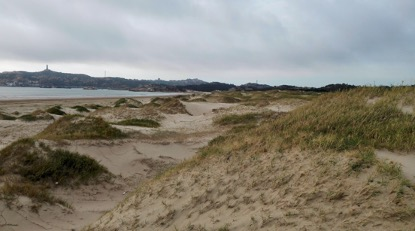
\includegraphics{../figs/sand_buried_plants.jpg}}}\hspace{5pt}
  \subfloat[\textit{C. equisetifolia} danmaged by sand burial.]{%
  \resizebox*{6cm}{!}{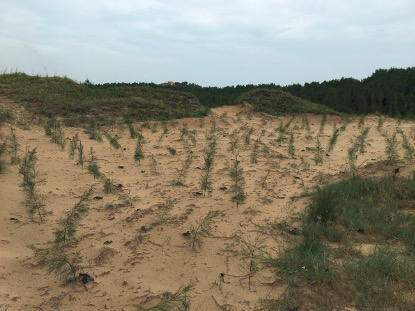
\includegraphics{../figs/damaged_trees.jpg}}}
  \caption{(a) Intensive sand burial on the Spinifex littoreus nebkhas on Pingtan island after typhoon Soudelor (1513) landed in Putian City, Fujian Province, China in August, 2015. (b)The nebkhas formed by Spinifex littoreus was stabilized by the planting of an invasive species Casuarinas equisetifolia seedlings on Pingtan Island, Fujian Province, China.} 
  \label{sample-pic}
\end{figure}

\label{Introduction-5}
% 我们的研究假设和研究思路
% 我们认为不同的沙埋情形将改变植株的生长方式,是该植物能够适应台风带来的强烈沙埋的关键性因素。
In this study, we assume that the different sand burial changes the growth process of S. littoreus, which is the key factor for the plants to adapt to the intense sand burial. Then, the vertical height of ramets, horizontal length of stolons, and biomass allocation of adventitious roots, stems and leaves on stolons of S. littoreus under different sand burial levels were simulated and measured in a field experiment, in a growing season on Pingtan Island, Fujian Province, South China.


\section{Material and Methods}
\subsection{Study area}

\begin{figure}
  \centering
  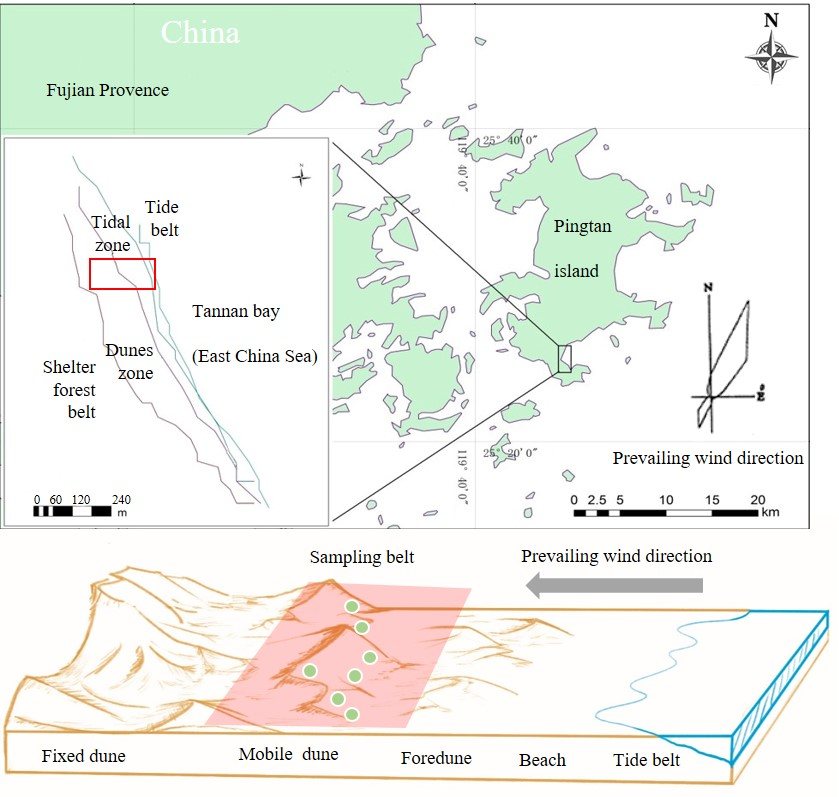
\includegraphics[scale=0.8]{../figs/study_area.jpg}
  \caption{Schematic diagram of the field experiment} 
  \label{fig:map}
\end{figure}

Pingtan island is located on the eastern coast of Fujian province, South China, with a sub-humid and oceanic monsoon climate. The study area is situated in the southeast of Pingtan island $(25^{\circ}26'36''-25^{\circ}26'48''N, 119^{\circ}46'09''-119^{\circ}46'21''E)$, and is usually regarded as hosting the most well-preserved coastal sand dunes in China (Figure~\ref{fig:map}) (Yang et al. 2017). Annual average temperature is 19.5℃, and precipitation is 1151 mm. The Monsoon is the dominant wind in this area, SE in the summer and NE in the winter, with an annual average wind speed of $6.9 m/s$. A total of 106 typhoons made landfall on Pingtan island from 1981 to 2019, average 2.65 times per year, and mainly they occur in July to September. The maximum wind speed can be up to $32.7 m/s$, ultimately leading to the severe sand burial on the psammophytes in this period. Soil is mainly composed of medium to fine sand, with well-sorted grains. Sediments are transported by the wind and intercepted by the ramets and stolons of S. littoreus, and a discrete dune mound or hummock was usually formed by aeolian sand deposition within an isolated plant or group of plants (Hesp \& Smyth 2019), ultimately developing into a 300 m wide nebkha dominated foredune zone (Figure~\ref{sample-pic}). S. littoreus is the dominant species in the study area and the auxiliary plants including Oenothera drummondii, Cynodondactylon, Pluchea pteropoda, and Sesuvium portulacastrum. 



\subsection{Methods}
Field experiments were carried out in July, 2016, in Tannan bay, Pingtan Island (Figure~\ref{fig:map}). One study belt without the interruption of animals, pollutants, and apparent human activities was selected in the center of the coastal sand dunes. Considering most of the S. littoreus were distributed on the windward slopes, 35 healthy plants with uniform size and comparable age were selected on the windward slopes were chosen for study. All the observed plants can be well distinguished from surrounding plants, and the height of vertical ramets and the length of stolons were all similar with each other before the burial treatments. Stolons of plants on the windward slopes were selected, and labeled with a red cord at points 1/3 and 2/3 of the length from the stem base to the apex of the stolons. Weeds around the selected plants were manually cleared, and wooden frames 20 cm in height (similar to the height of stolons) were set around the selected plants. Later, all the observed plants were fixed with a label, and its serial number was recorded on the label and wooden baffles respectively in order to facilitate periodic measurements later. The few adventitious roots present on the stolons of the observed plants were completely eliminated, the height of vertical ramets and length of stolons were measured separately before the experiments began. Later, all the plants were buried with sand from the nearby dunes according to a variety of different treatments (Figure 4). 


\begin{figure}
  \centering
  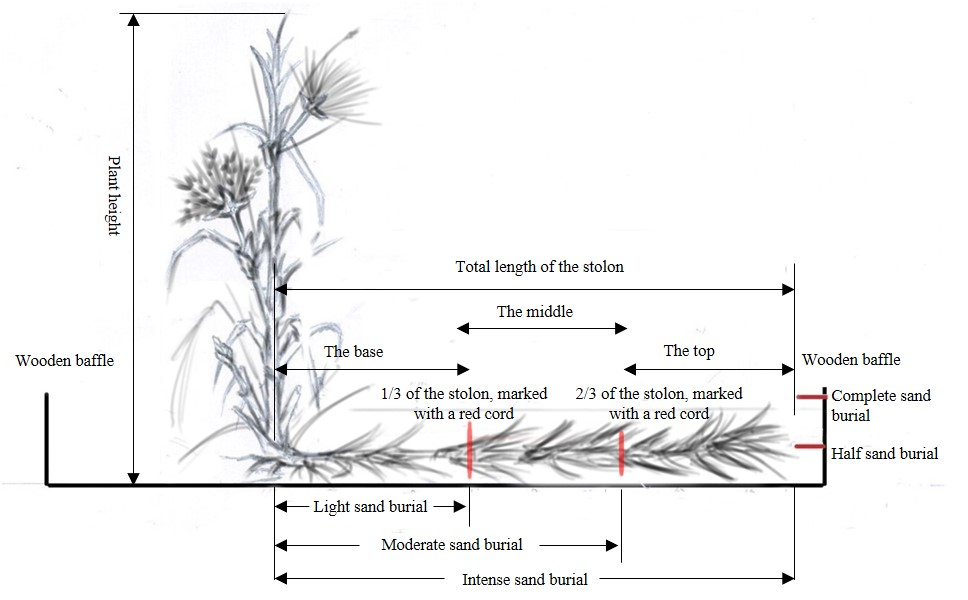
\includegraphics[scale=0.5]{../figs/diagram.jpg}
  \caption{Schematic diagram of the sand burial treatments of the samples} 
  \label{fig:diagram}
\end{figure}

\begin{table}
  \tbl{Sand burial treatments of the plants.}
  {\begin{tabular}{lrrr} 
  \toprule
   Treatment & Burial depth & Burial level \\ 
  \midrule
   CG & No sand burial & No sand burial \\
   HL & Half & Light \\
   HM & Half & Moderate \\
   HI & Half & Intense \\
   CL & Complete & Light \\
   CM & Complete & Moderate \\
   CI & Complete & Intense \\
  \bottomrule
  \end{tabular}}
  \label{tab:treatment}
\end{table}

While control groups (CG) had not been buried by sand artificially, and other groups were buried in different ways. Since the height of vertical ramets of S. littoreus is relatively high, it is naturally impossible for them to be completely buried in the sand. The treated S.littoreus, thus, only the stolons of which were buried at different depths and levels (see Figure~\ref{fig:diagram} and Table~\ref{tab:treatment}). Moreover, some adventitious roots on the stolons of selected plants were observed only a few days after sand burial, so the growth parameters of plants were dynamically investigated in 5, 9, 13, 17, 20 days after the sand burial to investigate the response of S.littoreus to severe sand burial over a short time scale.

During the measurements, the sand burying the plants was carefully removed to one side in a wooden baffle, and the height of the vertical ramets, the length of the stolons and adventitious roots were all measured with a tape. In the end, all the plants were buried again with the previous sand. When the experiments were finished, both above and below ground biomass of plants were collected and separated according to the label previously fixed on the stolons. Then all the samples were taken to the laboratory, and the roots, stems and leaves were separated from the stolons, dried in the oven with a temperature of 65℃ for about 24 h until the weight was constant, and then weighed with an analytical balance (accuracy: 0.0001g).

All the data were calculated with average according to all the replications with standard error as measurement of variability. The results were analysed with Python3 and package Pingouin. For each observed variable, we used repeated measure ANOVA analysis to test if the experimental treatments were verified due to time, and checked the significance $(P<0.05)$.

\section{Results}

\subsection{Influence of sand burial on growth processes of \textit{S. littoreus}}


\subsection{Influence of sand burial on the biomass allocation}


\section{Discussion}

\subsection{Mechanism of \textit{S. littoreus'} responses to severe sand burial}

\subsection{Significance of \textit{S. littoreus'} adaptation to sand burial}


\section*{Acknowledgement(s)}

An unnumbered section, e.g.\ \verb"\section*{Acknowledgements}", may be used for thanks, etc.\ if required and included \emph{in the non-anonymous version} before any Notes or References.


\section*{Disclosure statement}

An unnumbered section, e.g.\ \verb"\section*{Disclosure statement}", may be used to declare any potential conflict of interest and included \emph{in the non-anonymous version} before any Notes or References, after any Acknowledgements and before any Funding information.


\section*{Funding}

An unnumbered section, e.g.\ \verb"\section*{Funding}", may be used for grant details, etc.\ if required and included \emph{in the non-anonymous version} before any Notes or References.


\section*{Notes on contributor(s)}

An unnumbered section, e.g.\ \verb"\section*{Notes on contributors}", may be included \emph{in the non-anonymous version} if required. A photograph may be added if requested.


\section*{Nomenclature/Notation}

An unnumbered section, e.g.\ \verb"\section*{Nomenclature}" (or \verb"\section*{Notation}"), may be included if required, before any Notes or References.


\section*{Notes}

An unnumbered `Notes' section may be included before the References (if using the \verb"endnotes" package, use the command \verb"\theendnotes" where the notes are to appear, instead of creating a \verb"\section*").


\section{References}

test\citep{quEffectsSandBurial2017}

\bibliographystyle{tfcse.bst}
\bibliography{interactcsesample}

\end{document}
